\documentclass[11pt,a4paper]{article}

% --- XeLaTeX + Unicode Vietnamese ---
\usepackage{fontspec}
\setmainfont{DejaVu Serif}
\setsansfont{DejaVu Sans}
\setmonofont{DejaVu Sans Mono}
\usepackage[margin=1in]{geometry}
\usepackage{natbib}
\usepackage{booktabs}
\usepackage{graphicx}
\graphicspath{{figures/}}
\usepackage{hyperref}
\usepackage{xurl}
\usepackage{amsmath,amssymb}
\usepackage{enumitem}
\usepackage{xcolor}
\usepackage{microtype}
\usepackage{tabularx}
\usepackage{seqsplit}

\hypersetup{
  colorlinks=true,
  linkcolor=black,
  citecolor=blue,
  urlcolor=blue
}

% Compact lists
\setlist[itemize]{leftmargin=1.5em,itemsep=0.2em,topsep=0.3em}
\setlist[enumerate]{leftmargin=1.5em,itemsep=0.2em,topsep=0.3em}

\title{Unknown Outcomes and Authority-Aware Replay:\\
Tool-Boundary Semantics for Durable LLM Agents}

\author{
Nguyễn Mạnh Hùng$^{1}$\thanks{Corresponding author.} \and
Phạm Thị Minh Hồng$^{1}$ \and
Nghiêm Thị Mỹ Linh$^{1}$ \and
Phạm Thị Thu Thảo$^{1}$ \and
Nguyễn Tiến Long$^{1}$\\[0.5em]
\normalsize$^{1}$Vietnam Maritime University --- Faculty of Information Technology\\
\texttt{hungkhp888@gmail.com}
}

\date{September 18, 2026}

\begin{document}
\maketitle

% ============================================================
\begin{abstract}
Long-running LLM agents that mutate external state remain vulnerable at
tool boundaries: session or graph checkpoints restore conversation, but do
not prove which side effects already committed. After crash and restore,
models may re-synthesize tool arguments, causing duplicate payments,
notifications, or writes---Action Replay and Authority Resurrection
(ACRFence). We propose a local-first harness semantics that separates
transport from effect, keeps a ternary effect journal with an explicit
\texttt{unknown} state and reconciliation, and consumes artifact-bound
authority at confirmation. We formalize invariants I1--I5, map them onto
neko-core, and evaluate baselines B0--B3 on mock mutating tools under a
locked crash-injection protocol with fixed weights and mandatory
model--harness reporting. In a scripted pilot ($N{=}10$) and confirmatory LLM-in-the-loop
runs (glm-5.3 via z.ai, $N{=}30$ on F01/F02/F03$\times$M-pay$\times$\{B2,B3\}
plus F01$\times$M-fs$\times$\{B2,B3\} and F01$\times$M-mail$\times$\{B2,B3\};
300~cells, 76584~tokens, 0~failures), the
primary safety headlines remain B3~$\succ$~B2 on F01 duplicates under
re-synthesis ($0.0$ vs~$1.0$) and on F03 Authority Resurrection
($0.0$ vs~$1.0$). F01$\times$M-fs and F01$\times$M-mail replicate RQ1 using
\texttt{writes\_len} and \texttt{emails\_sent}, respectively;
F02 exposes a safety/completeness tradeoff rather than a universal B3
completeness win. A pinned neko-seal adapter ($N{=}30$, @\texttt{c863cc6}) reproduces
F01 RQ1 under the sealed restore path without closing scaffold$\neq$production.
Caveats: primary LLM empirics still run on an \texttt{eval-harness} scaffold
(journal/I5 lab-side); mock tools, a single model (\texttt{glm-5.3}), and
scripted faults. This Phase-1 preprint stakes claims
for feedback; it is not yet Q2 journal submit-ready. We do not replace
Temporal-style workflow engines or treat MCP support as novelty.
\end{abstract}

\noindent\textbf{Keywords:}
LLM agents; agent harness; durable execution; crash recovery;
tool-boundary semantics; unknown outcome; authority consumption;
Action Replay; Authority Resurrection; local-first systems

% ============================================================
\section{Introduction}
\label{sec:intro}

LLM agents that call mutating tools fail under crash and restore for a
reason that is easy to miss in chat-centric designs: a session or graph
checkpoint can restore \emph{what was said} without proving \emph{which
external effects already happened}. After restore, the model may
re-synthesize tool arguments. Servers then treat the new request as fresh
work, producing duplicate side effects---payments, notifications,
filesystem writes, deploy flags---even when the operator believed the run
had only ``resumed.'' ACRFence names the core threats as Action Replay and
Authority Resurrection: re-issuing a mutation without a receipt, and
reviving spent approval for a re-synthesized request
\cite{acrfence2026}. Classic idempotency keys help only when the
\emph{same} key is reused; they do not bind when the harness emits a new
identifier for a semantically related call \cite{beyondtokens2026}.

Practice and surveys already treat reliability as a \emph{harness}
problem. Guidance on long-running agent harnesses stresses cross-session
progress and clean handoff across context windows
\cite{anthropic2025harnesses}. Harness surveys place Lifecycle and
Governance beside Execution, and argue that bottlenecks may sit in the
harness as much as in the foundation model
\cite{li2026harnesssurvey,guo2026fromqa}. Durable-execution engines go
further: Temporal's Agent Harness offers an outer durable history and a
policy seam before tools \cite{temporal2026agentharness}, and systems
notes insist that checkpointing conversation state is not durable
execution of effects \cite{zylos2026durable}. What remains under-specified
for \textbf{local-first} agent development environments is a small,
measurable semantics at the \emph{tool boundary}: a ternary effect journal
that can enter \texttt{unknown}, refuse blind replay until reconcile, and
\textbf{consume} artifact-bound authority on confirm---without claiming to
replace workflow fleets.

\paragraph{Claim.}
Under intentional crash/restore at tool boundaries, and with model weights
fixed, a harness that (1)~separates transport from effect, (2)~keeps an
\texttt{unknown} control state with reconciliation, and (3)~consumes
authority at effect confirmation reduces duplicate external effects
relative to checkpoint-only and checkpoint+idempotency-key baselines on a
local-first stack (neko-core~/~wiii), addressing Action Replay and
Authority Resurrection. A scripted pilot ($N{=}10$) supports this: under
F01$\times$M-pay with argument re-synthesis, B3 achieves
\texttt{duplicate\_effect\_rate}~$0.0$ vs B2's~$1.0$
(E-20260918-17); under F03, B3 uniquely blocks Authority Resurrection
that B1/B2 exhibit (E-20260918-16). Confirmatory LLM cells
(\texttt{glm-5.3}, $N{=}30$, B2 vs B3) reproduce the same headlines:
F01 duplicate rates $1.0$ vs~$0.0$ (E-20260918-22) and F03 mean
authority resurrection $1.0$ vs~$0.0$ (E-20260918-23). The F01$\times$M-fs and F01$\times$M-mail replications give the same RQ1
separation on \texttt{writes\_len} and \texttt{emails\_sent}, respectively
(E-20260918-27/33), while F02 records the safety/completeness tradeoff
(E-20260918-28).

\paragraph{Contributions.}
\begin{enumerate}
\item \textbf{Formal tool-boundary effect model (I1--I5):}
pre-effect durability; unknown~$\neq$~success; no blind replay from
unknown; authority intersection narrow-only; authority consumption bound
to artifact hash---distinguishing chat memory, effect journal, and
procedural workflows \cite{awm2025}.
\item \textbf{Open realization on neko-core:}
lift existing pre-effect checkpoints and unknown seals into an explicit
effect journal and B3 baseline, with ADE/wiii as deployment context rather
than a second novelty claim.
\item \textbf{Crash-injection evaluation protocol:}
compare B0--B3 under a fault catalog aligned to ACRFence classes; report
model--harness pairs in the spirit of harness-aware eval
\cite{harnessbench2026,agencybench2026,hal2025}; primary metric =
duplicate external effects per injected fault.
\end{enumerate}

\paragraph{Non-goals (scope).}
We do not replace Temporal or Restate; MCP support is wire, not novelty;
we do not claim Phase-1 SWE-bench SOTA (mock mutating tools first).
Fine-grained permission trees \cite{ac4a2026} are related governance
context, not our primary claim. Venue ambition is a Q2 systems/SE journal
track (JSS as primary target); we do not print an unverified Scopus/JCR
quartile on a CV from this draft alone. An arXiv Phase-1 upload remains an
optional intermediate for claim staking, not the finish line.

\paragraph{Paper map.}
Section~\ref{sec:background} backgrounds harness durability and the threat
model. Section~\ref{sec:model} presents the effect state machine and
invariants I1--I5. Section~\ref{sec:system} maps the model onto neko-core.
Section~\ref{sec:methods} details baselines B0--B3, faults, and metrics.
Section~\ref{sec:results} reports scripted pilot results (incl.\
re-synthesis) and confirmatory LLM aggregates ($N{=}30$).
Section~\ref{sec:discussion} discusses limits, Q2-bar gaps, and local-first
positioning. Section~\ref{sec:related} relates prior work;
Section~\ref{sec:conclusion} concludes.

% ============================================================
\section{Background and Threat Model}
\label{sec:background}

\subsection{Harness durability vs.\ chat checkpoints}

Production writing already treats reliability as a harness concern
\cite{anthropic2025harnesses}. Survey work frames the same layer
systematically: Lifecycle and Governance sit beside Execution
\cite{li2026harnesssurvey}, and a model--harness lens argues that
bottlenecks may sit in harness design as much as in foundation models
\cite{guo2026fromqa}. Industry systems synthesis sharpens the distinction
between checkpointing and durable execution: session memory is not an
effect journal \cite{zylos2026durable}. Temporal's Agent Harness positions
an \emph{outer} harness with durable workflow history and a policy seam
before tool execution \cite{temporal2026agentharness}. We cite these as
baselines and as \textbf{non-replacements}: Angle~A studies lighter journal
semantics for local-first agent stacks, not a substitute for Temporal-style
workflow fleets.

\subsection{Threat classes (ACRFence)}

We align our fault catalog to ACRFence's named threats
\cite{acrfence2026}:
\begin{itemize}
\item \textbf{T-AR (Action Replay):} re-issuing a mutating call after
  restore without proving prior outcome.
\item \textbf{T-ARes (Authority Resurrection):} reviving spent approval
  for a re-synthesized request.
\item \textbf{T-FS (False Success):} harness reports success when the
  external effect did not commit (or disagrees with ground truth).
\item \textbf{T-LA (Lost Ack):} effect may have committed but durable
  receipt is missing---often the precursor to Action Replay.
\end{itemize}
Classic idempotency keys help only when the same key is reused; they fail
when the model re-synthesizes arguments and the harness mints a fresh key
\cite{beyondtokens2026}.

\subsection{Threat model (ACRFence-style)}
\label{sec:threat-model}

We follow ACRFence's early threat-model placement \cite{acrfence2026}: name
what we protect, who can force restore, which invariants we enforce, and
what is out of scope---before stating the effect machine.

\paragraph{Assets / what we protect.}
\begin{itemize}
\item \textbf{Effect-journal integrity:} after crash/restore, the harness
  must not treat a missing durable receipt as license for blind irreversible
  re-execution (transport~$\neq$~effect).
\item \textbf{Spent authority stays spent:} artifact-bound authority tokens
  $\kappa$ consumed at confirmation must not become re-usable after rewind
  (Authority Resurrection).
\item \textbf{No blind irreversible re-execution:} when outcome is
  \texttt{unknown}, the harness must reconcile against mock ground truth
  before confirming or re-issuing a mutating call.
\end{itemize}

\paragraph{Adversary models (aligned to ACRFence).}
\begin{enumerate}
\item \textbf{Crash-Induced Restore:} a crash after an irreversible mock
  effect (or after approval, before execute) causes the framework to restore
  a prior checkpoint; the agent (or scripted driver with
  \texttt{--resynthesize}) re-issues tool arguments that may differ from the
  pre-crash call---servers then treat the call as fresh work.
\item \textbf{Deliberate Rollback Abuse:} an operator with rewind/restore
  access intentionally restores to a post-approval or pre-receipt checkpoint
  to re-issue mutations or revive a spent $\kappa$. In scope as
  operator/rewind misuse of the harness control plane; \textbf{not} a
  malicious host OS, compromised kernel, or off-path network adversary.
\end{enumerate}

\paragraph{Invariants we enforce (tie to I2/I3/I5).}
We target the same safety spirit as ACRFence's two restore invariants,
expressed in our effect model:
\begin{itemize}
\item \textbf{I2/I3 --- no blind replay from unknown:}
  \texttt{unknown}~$\neq$~success; no second irreversible effect until
  reconcile inspects counters/hashes.
\item \textbf{I5 --- consumed artifact-bound authority stays consumed:}
  after confirm, $\kappa$ bound to
  $\mathrm{hash}(t,\,a_{\mathrm{canonical}},\,\mathrm{artifact})$ cannot
  authorize a re-synthesized or restored call without fresh approval.
\end{itemize}

\paragraph{Assumptions.}
(i)~Mutating tools in reported runs are \textbf{mock-instrumented} so
counters and artifact hashes are ground truth; (ii)~model weights (or the
scripted driver) are \textbf{fixed} across baseline ablations so differences
attribute to harness policy; (iii)~crash injection is confined to the
mock/registry boundary under the locked fault catalog; (iv)~no real
payments, SMTP, or production deploys.

\paragraph{Out of scope (non-goals).}
Malicious host / TEE restart; model-weight or prompt-injection attacks as
primary threat; real payment/SMTP/deploy endpoints; replacing Temporal-class
workflow fleets; treating MCP wire support as novelty; Phase-1 SWE-bench
SOTA claims.

% ============================================================
\section{Effect Model}
\label{sec:model}

LLM agents re-synthesize tool arguments after restore. Session/graph
checkpoints therefore do \textbf{not} imply exactly-once external effects.
We formalize a small effect state machine suitable for RQ1/RQ2 evaluation.

\subsection{Objects}

\begin{center}
\begin{tabular}{@{}ll@{}}
\toprule
Symbol & Meaning \\
\midrule
$M$ & Fixed foundation model (weights/config pinned) \\
$H$ & Harness (neko-core runtime + host gates) \\
$t$ & Tool name / MCP tool id \\
$a$ & Tool arguments (possibly re-synthesized) \\
$e$ & Effect record id (stable across restore) \\
$r$ & Durable receipt / observation \\
$\kappa$ & Authority token bound to artifact hash \\
$\sigma$ & Session checkpoint (messages, mode, profile, \ldots) \\
$J$ & Effect journal (confirmed / rejected / unknown) \\
\bottomrule
\end{tabular}
\end{center}

\noindent\textbf{Vocabulary distinction.}
Conversation/session memory $\subset \sigma$ (what was said); effect
journal $J$ (which mutations are confirmed/rejected/unknown); procedural
workflows (AWM-style) are reusable how-to text, \textbf{not} control-flow
durability \cite{awm2025}.

\subsection{Effect state machine}

Each irreversible (or potentially irreversible) tool admission creates an
effect $e$ with states:
\begin{itemize}
\item \textbf{proposed} --- model requested $t(a)$; $\kappa$ not yet
  consumed.
\item \textbf{executing} --- pre-effect checkpoint written; side effect may
  be in flight.
\item \textbf{confirmed} --- durable receipt $r$ proves completion;
  $\kappa$ \textbf{consumed}.
\item \textbf{rejected} --- denied by gate/policy or failed closed before
  external commit.
\item \textbf{unknown} --- pre-effect durable intent exists, no durable
  receipt.
\item \textbf{reconciling} --- subphase of unknown: inspect world state
  before any new mutation.
\end{itemize}
Transitions of interest: crash/abort/timeout from \texttt{executing} enter
\texttt{unknown}; reconcile may move \texttt{unknown}$\to$\texttt{confirmed}
(world shows done) or \texttt{unknown}$\to$\texttt{rejected} (absent +
safe). Fork to a new proposed effect requires fresh $\kappa'$ bound to
possibly new args---never resurrecting spent $\kappa$.
Figure~\ref{fig:effect-sm} summarizes the machine.

\begin{figure}[t]
\centering
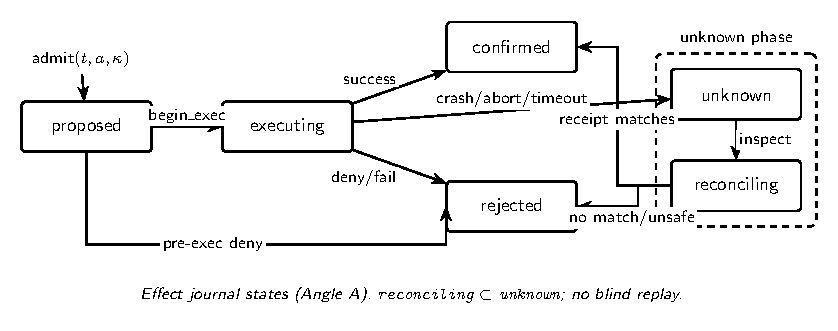
\includegraphics[width=\linewidth]{effect-state-machine.pdf}
\caption{Effect journal state machine: \texttt{proposed}$\to$\texttt{executing}
  then \texttt{confirmed}, \texttt{rejected}, or \texttt{unknown}; \texttt{reconciling}
  is a subphase of \texttt{unknown} (inspect before any new mutation).}
\label{fig:effect-sm}
\end{figure}

\subsection{Invariants (I1--I5)}

\begin{description}[style=nextline,leftmargin=2.2em]
\item[I1 --- Pre-effect durability.]
Before invoking a mutating tool body, $H$ persists enough of $\sigma$ that
a crash yields a recoverable in-flight record.
\item[I2 --- Unknown $\neq$ success.]
An interrupted mutation is never labeled success; sealed content instructs
inspect-before-retry.
\item[I3 --- No blind replay from unknown.]
Transition \texttt{unknown}$\to$\texttt{executing} with a \textbf{new}
effect id $e'$ is forbidden until reconcile completes.
\item[I4 --- Authority intersection (narrow-only).]
Effective permission $= \cap\{\text{tool class},\,\text{mode},\,\text{turn
lease},\,\text{launch authority}\}$. Intersection may narrow, never expand
host policy.
\item[I5 --- Authority consumption (RQ2).]
$\kappa$ is bound to $\mathrm{hash}(t,\,a_{\mathrm{canonical}},\,\mathrm{artifact})$;
confirmation consumes $\kappa$. Restore must not revive a consumed $\kappa$
for a re-synthesized $a'$ (Authority Resurrection).
\end{description}
Optional \textbf{I6} (provider semantic commit: transport retry may be safe
before visible output; after committed semantic event, continue from
checkpoint rather than blind HTTP replay) is implementation context, not
the paper's primary claim.

\subsection{Threat alignment}

\begin{center}
\small
\begin{tabularx}{\linewidth}{@{}l>{\raggedright\arraybackslash}X>{\raggedright\arraybackslash}X@{}}
\toprule
Attack class & Machine reading & Mitigated by \\
\midrule
Action Replay &
  unknown/executing $\to$ new side effect without reconcile &
  I2, I3, B3 reconcile \\
Authority Resurrection &
  consumed $\kappa$ reused for $a'$ &
  I5 \\
Semantic re-synthesis &
  $a' \neq a$ treated as retry &
  I3 fork + new $\kappa'$; B2 alone insufficient \\
\bottomrule
\end{tabularx}
\end{center}

% ============================================================
\section{System Realization}
\label{sec:system}

We realize the model on the local-first \texttt{neko-core} stack, with
ADE/\texttt{wiii} as deployment context rather than a second treatment.

\begin{center}
\footnotesize
\begin{tabularx}{\linewidth}{@{}>{\raggedright\arraybackslash}p{0.22\linewidth}>{\raggedright\arraybackslash}X>{\raggedright\arraybackslash}X@{}}
\toprule
Formal piece & Already in neko-core & Contribution for paper \\
\midrule
Pre-effect checkpoint &
  Yes (\texttt{durableCheckpoint} before tool) &
  Measure under crash injection \\
Unknown seal &
  Yes (dangling tool\_call; \texttt{unknown\_outcome}) &
  Lift to first-class journal state $e$ \\
Non-auto-replay &
  Yes (docs + stop policy) &
  Enforce in eval harness B3 \\
Authority $\cap$ &
  Yes (modes, leases, profiles) &
  Add consume-on-confirm + artifact hash \\
Effect journal $J$ &
  Partial (trajectory embeds results) &
  Explicit receipt store for mocks \\
Reconcile probes &
  Advised in text &
  Automated reconcileor for mock tools \\
\bottomrule
\end{tabularx}
\end{center}

\noindent Audit notes (2026-09-18): neko-core already checkpoints before
managed tool execution and can seal interrupted mutations; MCP failures may
return ``outcome unknown; not retried.'' Gaps relative to a full machine
include: no first-class effect id spanning proposed$\to$confirmed across
tools; \texttt{unknown\_outcome} is often convention rather than one shared
enum; reconciling is policy text more than an enforced phase; and I5
single-consume tokens bound to artifact hash are the clearest net-new
mechanism measured in the B3 scaffold.

% ============================================================
\section{Methods}
\label{sec:methods}

\subsection{Overview}

We evaluate whether a tool-boundary harness with ternary effect state and
single-consume authority reduces \textbf{duplicate external effects} under
intentional crash/restore, relative to checkpoint baselines, with
\textbf{model weights fixed}. Threats follow ACRFence
\cite{acrfence2026}. All mutating side effects run through \textbf{mock
tools} only. Every reported cell identifies a \textbf{model--harness pair}
\cite{harnessbench2026}.

\subsection{Baselines}

\begin{center}
\begin{tabular}{@{}lll@{}}
\toprule
ID & Tag & Recovery policy \\
\midrule
B0 & \texttt{none} &
  No durable session; crash $\Rightarrow$ cold start \\
B1 & \texttt{session\_ckpt} &
  Persist trajectory; resume may re-drive in-flight tools \\
B2 & \texttt{ckpt\_idem} &
  B1 + client idempotency key on every mock mutating call \\
B3 & \texttt{unknown\_auth} &
  B1 + seal-unknown + reconcile + authority consume (RQ2) \\
\bottomrule
\end{tabular}
\end{center}

B3 realizes the formal machine: transport~$\neq$~effect; interrupted
mutations seal as \texttt{unknown}; reconcile inspects mock ground truth
before any new mutate; spent authority cannot authorize a re-synthesized
request.

\subsection{Mock tools}

\begin{center}
\begin{tabular}{@{}lll@{}}
\toprule
Mock ID & Tool & Observable side effect \\
\midrule
M-pay & \texttt{mock\_payment\_charge} &
  \texttt{charge\_count}, \texttt{charges[]} \\
M-mail & \texttt{mock\_email\_notify} &
  \texttt{emails\_sent} \\
M-fs & \texttt{mock\_fs\_write} &
  \texttt{writes[]}, file bytes, content hash \\
M-flag & \texttt{mock\_deploy\_flag} &
  \texttt{flag\_set\_count}, flag value \\
\bottomrule
\end{tabular}
\end{center}

Mocks expose deterministic seeds, counter read APIs, optional
\texttt{idempotency\_key}, optional \texttt{authority\_token} (B3), and
crash hooks. Ground truth is mock counters / artifact hashes, not model
self-report.

\subsection{Fault catalog (F01--F10)}

Injection points sit at mock / \texttt{ToolRegistry} boundaries.

\begin{center}
\footnotesize
\begin{tabularx}{\linewidth}{@{}l>{\raggedright\arraybackslash}X>{\raggedright\arraybackslash}p{0.14\linewidth}>{\raggedright\arraybackslash}X@{}}
\toprule
ID & Injection (summary) & Threat & B3 expectation \\
\midrule
F01 & Kill after mock success, before durable receipt &
  T-LA$\to$T-AR & Seal unknown; reconcile; no second effect \\
F02 & Kill mid-mutation &
  T-LA / T-FS & \texttt{unknown}$\to$reconciling; inspect \\
F03 & Restore after approval, before execute &
  T-ARes & Authority bound to artifact+effect; else re-approve \\
F04 & After confirm, model re-synthesizes same intent &
  T-AR & Consumed authority + ledger reject \\
F05 & Duplicate resume with spent authority &
  T-ARes & Single-consume deny \\
F06 & Transport retry after semantic commit &
  T-AR & Transport retry $\neq$ effect retry \\
F07 & Crash during reconcile of unknown &
  T-AR / T-FS & Sticky unknown until inspect completes \\
F08 & Idempotency key present; harness still replays &
  T-AR / T-FS & No second execute when reconciled confirmed \\
F09 & FS write commits; session checkpoint lags &
  T-LA$\to$T-AR & Reconcile by content hash \\
F10 & Payment double-charge under B1 (headline RQ1) &
  T-AR & Reconcile \texttt{charge\_count}; no second charge \\
\bottomrule
\end{tabularx}
\end{center}

\begin{figure}[t]
\centering
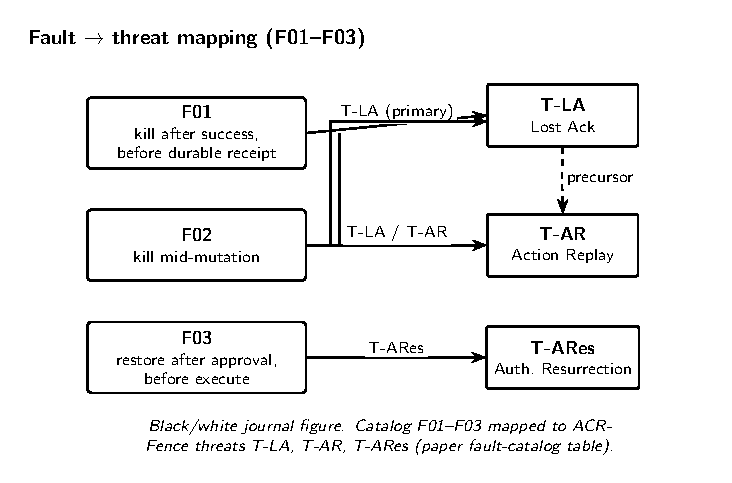
\includegraphics[width=0.95\linewidth]{threat-map.pdf}
\caption{Mapping of primary eval faults F01--F03 to ACRFence threat classes
  T-LA (Lost Ack), T-AR (Action Replay), and T-ARes (Authority Resurrection).
  F01 is T-LA$\to$T-AR; F02 engages T-LA/T-AR under mid-mutation; F03 is T-ARes.}
\label{fig:threat-map}
\end{figure}


\subsection{Experimental design}

A \textbf{cell} $= (\text{baseline} \times \text{fault\_id} \times
\text{mock\_id})$ with fixed $(\text{model\_id},\,\text{harness\_id})$.
Full catalog: $4 \times 10 \times 4 = 160$ cells. Pilot subset
(engineering-time): M-pay + M-fs $\times$ \{F01, F02, F03, F06, F09, F10\}
$\times$ B0--B3 $= 48$ cells. Meaningless fault$\times$mock pairs are
recorded NA with reason---never filled with invented outcomes.

\paragraph{Sample size.}
Pilot $N{=}10$ per cell (scripted driver). Confirmatory $N{=}30$ per cell
on F01/F02/F03$\times$M-pay and F01$\times$\{M-fs,M-mail\}, each with
$\{B2,B3\}$, uses an LLM driver (\texttt{glm-5.3},
\texttt{reasoning\_effort=low}, \texttt{resynthesize=true}); Wilson score
$95\%$ CIs are reported in Section~\ref{sec:results-confirm}; bootstrap remains
optional.

\paragraph{Single-run procedure.}
(1)~Start harness in baseline mode; register mocks on the sole effect path.
(2)~Fixed user task requiring one logical mutating effect.
(3)~Arm injector for \texttt{fault\_id}.
(4)~On crash, write marker; restore per baseline.
(5)~Recover to terminal state or timeout; record latency.
(6)~Read counters/hashes; write \texttt{meta.json}.
(7)~Reset mock state. For B3: missing durable result $\Rightarrow$ seal
unknown $\Rightarrow$ inspect $\Rightarrow$
\texttt{reconciling}$\to$\texttt{confirmed}$|$\texttt{rejected}; consume
authority only on confirm.

\subsection{Metrics}

\begin{center}
\small
\begin{tabularx}{\linewidth}{@{}>{\raggedright\arraybackslash}p{0.38\linewidth}>{\raggedright\arraybackslash}Xl@{}}
\toprule
Metric & Definition & Role \\
\midrule
\texttt{duplicate\_effect\_rate} &
  Fraction of runs with mock counter increment ${>}1$ &
  Primary (RQ1) \\
\texttt{false\_success\_rate} &
  Harness confirms success but mock disagrees &
  Safety \\
\texttt{recovery\_latency\_ms} &
  Restore start $\to$ stable terminal state &
  Cost \\
\texttt{re\_approval\_rate} &
  Fraction needing new gate approval after restore &
  RQ2 / UX \\
\texttt{authority\_resurrection\_count} &
  Attempts to execute with a \textbf{spent} token &
  RQ2 \\
\bottomrule
\end{tabularx}
\end{center}

\subsection{Model--harness reporting}

Every run and aggregate row reports
\texttt{model\_id}, \texttt{harness\_id}, \texttt{baseline},
\texttt{fault\_id}, \texttt{mock\_id}, \texttt{run\_id}, and
\texttt{evidence\_id} (harness id is e.g.\ \texttt{neko-core} at a git
SHA, or a scaffold id). Pilot cells use
\texttt{scripted/always-issue-tool} (optionally with
\texttt{--resynthesize}). Confirmatory cells use driver
\texttt{llm}, model \texttt{glm-5.3} (\texttt{model\_id}
\texttt{llm/glm-5.3@z.ai}), \texttt{reasoning\_effort=low}, harness
\texttt{eval-harness@scaffold}, and LLM Action Replay
(\texttt{resynthesize=true}). We do not pool across different harness
ids without an explicit harness factor \cite{harnessbench2026}. Artifact
layout: \texttt{evidence/runs/}\textit{E-id}\texttt{/} with
\texttt{meta.json}, crash markers, and pre/post counters.

\subsection{Exclusions and integrity}

Mocks only; no real money, SMTP, or production deploy. No
Temporal/workflow-engine replacement claim; MCP is not the contribution.
\textbf{No invented run numbers.} Pilot evidence for F01--F03 ($N{=}10$,
scripted) and confirmatory LLM evidence for F01/F02/F03$\times$M-pay
plus F01$\times$M-fs and F01$\times$M-mail ($N{=}30$, glm-5.3) are reported in
Section~\ref{sec:results}.

% ============================================================
\section{Evaluation and Results}
\label{sec:results}

\paragraph{Setup reminder.}
Pilot cells use fixed scripted policy
(\texttt{scripted/always-issue-tool} at scaffold), seeds 1--10,
faults from the locked catalog, and baselines B0--B3. Confirmatory cells
use an LLM driver (\texttt{glm-5.3}) on F01/F02/F03$\times$M-pay,
F01$\times$M-fs, and F01$\times$M-mail, each with $\{B2,B3\}$ ($N{=}30$, seeds 1--30). Harness:
\texttt{eval-harness} (scaffold).
Ground truth is mock counters. Date: 2026-09-18 ICT.
Evidence aggregates (filenames under \texttt{evidence/runs/}):
\begin{itemize}\setlength{\itemsep}{0pt}
\item \texttt{pilot-F01-Mpay-N10-summary.json} (E-20260918-16)
\item \texttt{pilot-F01-Mfs-N10-summary.json} (E-20260918-16)
\item \texttt{pilot-F02-Mpay-N10-summary.json} (E-20260918-16)
\item \texttt{pilot-F03-Mpay-N10-summary.json} (E-20260918-16)
\item \texttt{pilot-F01-Mpay-resynth-N10-summary.json} (E-20260918-17)
\item \texttt{confirmatory-llm-F01-Mpay-N30-summary.json}
  (E-20260918-22)
\item \texttt{confirmatory-llm-F01-Mfs-N30-summary.json}
  (E-20260918-27)
\item \texttt{confirmatory-llm-F01-Mmail-N30-summary.json}
  (E-20260918-33)
\item \texttt{confirmatory-llm-F02-Mpay-N30-summary.json}
  (E-20260918-28)
\item \texttt{confirmatory-llm-F03-Mpay-N30-summary.json}
  (E-20260918-23)
\item \texttt{confirmatory-neko-seal-F01-Mpay-N30-summary.json}
  (E-20260918-31)
\end{itemize}

\subsection{F01 --- Kill after success, before durable receipt}

\paragraph{M-pay (\texttt{mock\_payment\_charge}).}

\begin{center}
\begin{tabular}{@{}lrrr@{}}
\toprule
Baseline & \texttt{dup\_rate} & mean \texttt{charge\_count} &
  \texttt{seal\_unknown} \\
\midrule
B0 & 1.0 & 2.0 & 0.0 \\
B1 & 1.0 & 2.0 & 0.0 \\
B2 & 0.0 & 1.0 & 0.0 \\
B3 & 0.0 & 1.0 & 1.0 \\
\bottomrule
\end{tabular}
\end{center}

\paragraph{M-fs (\texttt{mock\_fs\_write}).}
Same pattern: B0/B1 duplicate rate $1.0$ (mean writes $2.0$); B2/B3 $0.0$
(mean writes $1.0$); B3 \texttt{seal\_unknown\_rate} $1.0$.

\paragraph{Reading.}
Under F01 with a \emph{stable} scripted retry, classic idempotency (B2)
already suppresses duplicate counters. B3 matches B2 on duplicates while
\textbf{always emitting} an unknown seal before reconcile---visible
instrumentation of I2/I3 that B2 lacks.

\subsection{F02 --- Kill mid-mutation (M-pay)}

\begin{center}
\begin{tabular}{@{}lrrr@{}}
\toprule
Baseline & \texttt{dup\_rate} & mean \texttt{charge\_count} &
  \texttt{seal\_unknown} \\
\midrule
B0 & 0.0 & 1.0 & 0.0 \\
B1 & 0.0 & 1.0 & 0.0 \\
B2 & 0.0 & 1.0 & 0.0 \\
B3 & 0.0 & \textbf{0.0} & 1.0 \\
\bottomrule
\end{tabular}
\end{center}

\paragraph{Reading.}
No baseline produced a \emph{counted} duplicate under this scaffold's
mid-body kill+retry model ($N{=}10$). B3 uniquely keeps
\texttt{seal\_unknown} and ends with \textbf{zero} confirmed charges after
reconcile when the mock left no committed receipt---conservative I2
(unknown~$\neq$~success). B0--B2 still report mean \texttt{charge\_count}
$1.0$ (retry completed a charge without an unknown seal). This is a
behavioral distinction, not a duplicate-rate win.

\subsection{F03 --- Restore after approval, before execute (RQ2)}

\paragraph{M-pay.}

\begin{center}
\begin{tabular}{@{}lrrr@{}}
\toprule
Baseline & \texttt{dup\_rate} & mean auth.\ resurrection &
  mean \texttt{charge\_count} \\
\midrule
B0 & 0.0 & 0.0 & 1.0 \\
B1 & 0.0 & \textbf{1.0} & 1.0 \\
B2 & 0.0 & \textbf{1.0} & 1.0 \\
B3 & 0.0 & \textbf{0.0} & \textbf{0.0} \\
\bottomrule
\end{tabular}
\end{center}

\paragraph{Reading.}
This is the clearest B3~$\succ$~B2 signal in the pilot: session checkpoint
and idempotency keys do \textbf{not} stop Authority Resurrection after
restore-before-execute (mean resurrection count $1.0$ on B1/B2). B3 refuses
to consume a mismatched/spent path, records resurrection $0.0$, and
performs \textbf{no} charge without fresh authority
(\texttt{charge\_count}~$0.0$)---aligning with I5 and RQ2
(E-20260918-16).

\subsection{F01 under semantic re-synthesis (B2 vs B3)}

\paragraph{Driver.}
\texttt{--resynthesize} mutates idempotency-relevant args on retry (e.g.\
payment \texttt{amount + attempt}) and mints a new idempotency key---an
ACRFence-style Action Replay case when the model does not reuse keys.
Model id: \texttt{scripted/always-issue-tool+resynth@scaffold}.
$N{=}10$, seeds 1--10 (E-20260918-17).

\begin{center}
\begin{tabular}{@{}lrrr@{}}
\toprule
Baseline & \texttt{dup\_rate} & mean \texttt{charge\_count} &
  \texttt{seal\_unknown} \\
\midrule
B2 (ckpt + idem.\ key) & \textbf{1.0} & 2.0 & 0.0 \\
B3 (unknown + reconcile + auth.) & \textbf{0.0} & 1.0 & 1.0 \\
\bottomrule
\end{tabular}
\end{center}

\paragraph{Reading.}
When retry arguments change, B2's idempotency keys no longer collide---
duplicate charges return (rate $1.0$). B3 still seals unknown and reconciles
against the already-committed mock effect, so counters stay at $1.0$. This
is the primary \textbf{RQ1} separation of B3 from B2 under the threat model
that motivates the paper (E-20260918-17).

\subsection{Confirmatory LLM (glm-5.3, $N{=}30$)}
\label{sec:results-confirm}

\paragraph{Driver.}
\texttt{--driver llm --model glm-5.3 --reasoning-effort low}
(implies \texttt{--resynthesize}): the live model proposes post-crash
tool arguments and a fresh idempotency key (Action Replay path).
Model id: \texttt{llm/glm-5.3@z.ai}; harness:
\texttt{eval-harness@scaffold}. Matrix: F01/F02/F03$\times$M-pay$\times$\{B2,B3\},
F01$\times$M-fs$\times$\{B2,B3\}, and F01$\times$M-mail$\times$\{B2,B3\},
each with seeds~1--30 ($300$~cells, $0$~failures). Per-mock LLM usage:
M-pay has $44913$ total tokens (F01:~$15283$; F02:~$14683$; F03:~$14947$),
M-fs has $16355$ total tokens (F01:~$16355$), and M-mail has $15316$
total tokens (F01:~$15316$); overall $76584$ total tokens.
Binary rates below report exact $k/n$ with Wilson score 95\% confidence
intervals ($z{=}1.96$); see also \texttt{outline/stats-ci-table.md}.

\paragraph{F01$\times$M-pay (E-20260918-22).}
\begin{center}
\small
\begin{tabular}{@{}lrrrrr@{}}
\toprule
Baseline & $k/n$ & \texttt{dup\_rate} & Wilson 95\% CI &
  mean \texttt{charge\_count} & \texttt{seal\_unknown} \\
\midrule
B2 & $30/30$ & \textbf{1.000} & $[0.886,\,1.000]$ & \textbf{2.0} & $0/30$ \\
B3 & $0/30$ & \textbf{0.000} & $[0.000,\,0.114]$ & \textbf{1.0} & $30/30$ \\
\bottomrule
\end{tabular}
\end{center}
Wilson score intervals on exact cell counts (binomial). B2 ends
\texttt{confirmed}$\times$30 with two charges; B3 seals unknown,
reconciles, and ends \texttt{confirmed\_via\_reconcile}$\times$30 with one
charge---matching the scripted re-synthesis pilot at larger $N$
(F01 LLM grand total $15283$ tokens; B2~$7585$, B3~$7698$).

\paragraph{F01$\times$M-fs (E-20260918-27).}
\begin{center}
\small
\begin{tabular}{@{}lrrrrr@{}}
\toprule
Baseline & $k/n$ & \texttt{dup\_rate} & Wilson 95\% CI &
  mean \texttt{writes\_len} & \texttt{seal\_unknown} \\
\midrule
B2 & $30/30$ & \textbf{1.000} & $[0.886,\,1.000]$ & \textbf{2.0} & $0/30$ \\
B3 & $0/30$ & \textbf{0.000} & $[0.000,\,0.114]$ & \textbf{1.0} & $30/30$ \\
\bottomrule
\end{tabular}
\end{center}
On the filesystem mock, the same B3~$\succ$~B2 separation appears under
Action Replay when the effect metric is \texttt{writes\_len}: duplicate
rate $0.000$ vs~$1.000$ (Wilson CIs as above) and mean writes length
$1.0$ vs~$2.0$ (LLM tokens B2~$8184$, B3~$8171$). The M-fs charge
count remains zero, so it is not the effect metric here.

\paragraph{F01$\times$M-mail (E-20260918-33).}
\begin{center}
\small
\begin{tabular}{@{}lrrrrr@{}}
\toprule
Baseline & $k/n$ & \texttt{dup\_rate} & Wilson 95\% CI &
  mean \texttt{emails\_sent} & \texttt{seal\_unknown} \\
\midrule
B2 & $30/30$ & \textbf{1.000} & $[0.886,\,1.000]$ & \textbf{2.0} & $0/30$ \\
B3 & $0/30$ & \textbf{0.000} & $[0.000,\,0.114]$ & \textbf{1.0} & $30/30$ \\
\bottomrule
\end{tabular}
\end{center}
On the mail mock, the effect metric is \texttt{emails\_sent}, not
\texttt{charge\_count} (charge count is $0$ for both baselines). B2 duplicates
all 30 cells, while B3 seals and reconciles all 30; errors are $0$ in both
baselines. The separation matches M-pay and M-fs (LLM tokens B2~$7697$,
B3~$7619$; grand total~$15316$).

\paragraph{F02$\times$M-pay (E-20260918-28).}
\begin{center}
\small
\begin{tabular}{@{}lrrrr@{}}
\toprule
Baseline & dup $k/n$ (Wilson CI) & mean \texttt{charge\_count} &
  seal $k/n$ & outcome \\
\midrule
B2 & $0/30$ $[0.000,\,0.114]$ & 1.0 & $0/30$ & confirmed$\times$30 \\
B3 & $0/30$ $[0.000,\,0.114]$ & 0.0 & $30/30$ & rejected\_via\_reconcile$\times$30 \\
\bottomrule
\end{tabular}
\end{center}
F02 shows the safety/completeness tradeoff (LLM tokens B2~$7321$, B3~$7362$).
B3 conservatively seals \texttt{unknown} and refuses blind replay, so
reconciliation ends in \texttt{rejected\_via\_reconcile}$\times$30 and may
drop the effect; B2 retries and completes one charge per cell. Thus B3 is
safer against Action Replay but is not a universal completeness win.
Duplicate rates are both $0/30$; the separation is seal + charge count.

\paragraph{F03$\times$M-pay (E-20260918-23).}
\begin{center}
\small
\begin{tabular}{@{}lrrrrr@{}}
\toprule
Baseline & $k/n$ & auth.\ res.\ rate & Wilson 95\% CI &
  mean \texttt{charge\_count} & outcome \\
\midrule
B2 & $30/30$ & \textbf{1.000} & $[0.886,\,1.000]$ & \textbf{1.0} & confirmed$\times$30 \\
B3 & $0/30$ & \textbf{0.000} & $[0.000,\,0.114]$ & \textbf{0.0} & re\_approval\_required$\times$30 \\
\bottomrule
\end{tabular}
\end{center}
Authority-resurrection rate is the fraction of cells with
\texttt{authority\_resurrection\_count}$>0$ (equals mean count here).
B3 blocks Authority Resurrection under LLM resume ($0.000$ vs~$1.000$) with
zero post charges (F03 LLM grand total $14947$ tokens; B2~$7477$, B3~$7470$).
Both baselines report \texttt{seal\_unknown} $0/30$ on F03.

\paragraph{Reading.}
Live glm-5.3 Action Replay reproduces the pilot RQ1/RQ2 separations on
the B2/B3 headline cells. The F01$\times$M-fs and F01$\times$M-mail results
give the same B3~$\succ$~B2 reading via \texttt{writes\_len} and
\texttt{emails\_sent}, respectively; F02 instead exposes the
safety/completeness tradeoff described above. Scope is intentionally narrow:
single model, scaffold harness, mock tools, and F01/F02/F03$\times$M-pay plus
F01$\times$\{M-fs,M-mail\}$\times$\{B2,B3\} only---not F04--F10 or B0/B1.

\subsection{Confirmatory neko-core seal path (F01$\times$M-pay, $N{=}30$)}
\label{sec:results-neko-seal}

\paragraph{Driver and pin.}
This subsection is \textbf{separate} from the glm-5.3 scaffold tables above
(do not mix \texttt{harness\_id} rows). Driver:
\texttt{scripted/neko-seal-fixture@adapter} (CLI
\texttt{confirmatory-neko-seal.ts})---\emph{not} \texttt{glm-5.3}.
Harness id:
\path{neko-core@c863cc6+eval-adapter@14cd188}, with
neko-core pinned at short \texttt{c863cc6} (full
\path{c863cc6a386f8eea048089a7276d619353de94b6}).
Restore seals dangling tool calls via real
\texttt{Agent.sealDanglingToolCalls}; EffectJournal/I5 and mocks remain
lab-side (dual-stack). Evidence: E-20260918-31;
\texttt{confirmatory-neko-seal-F01-Mpay-N30-summary.json}.

\paragraph{F01$\times$M-pay (E-20260918-31).}
\begin{center}
\small
\begin{tabular}{@{}lrrrrr@{}}
\toprule
Baseline & $k/n$ & \texttt{dup\_rate} & Wilson 95\% CI &
  mean \texttt{charge\_count} & \texttt{seal\_unknown} \\
\midrule
B2 & $30/30$ & \textbf{1.000} & $[0.886,\,1.000]$ & \textbf{2.0} & $30/30$ \\
B3 & $0/30$ & \textbf{0.000} & $[0.000,\,0.114]$ & \textbf{1.0} & $30/30$ \\
\bottomrule
\end{tabular}
\end{center}
B2 ends with outcome \path{blind_replay_invoked}$\times 30$
(errors~$0$); B3 ends with \path{confirmed_via_reconcile}$\times 30$
(errors~$0$).
Both report \path{seal_text_matches_neko_core_rate}~$1.0$.
Dup/charge matches the scaffold LLM F01 pattern
(\path{matches_scaffold_dup_charge_pattern=true}; E-20260918-22).

\paragraph{Reading (honesty).}
B2 \texttt{seal\_unknown}~$1.0$ here because restore \emph{always} runs
real \texttt{Agent.sealDanglingToolCalls}---this \textbf{differs} from
scaffold B2 seal~$0$ (E-20260918-22) and is \emph{not} a contradiction of
the RQ1 dup/charge pattern. Remaining fidelity gaps: dual-stack
(EffectJournal/I5 + mocks still lab-side); no full ACP session/load; no
\texttt{Provider.complete}/\texttt{runLoop}; crash = in-process
\texttt{CrashSignal}; no ToolRegistry production-mocks claim.
This partially addresses Q2 P0-1 (scaffold~$\neq$~production) but does
\emph{not} close it fully (Section~\ref{sec:q2-bar}).

\subsection{Cross-fault summary}

\begin{center}
\begin{tabular}{@{}llll@{}}
\toprule
Fault & Where B0/B1 fail & Where B2 helps & Where B3 uniquely helps \\
\midrule
F01 & duplicate counters & yes (same key) &
  seal+reconcile (parity on dups) \\
F01+resynth & --- & \textbf{no} &
  \textbf{no duplicate} ($0$ vs $1$) \\
F02 & (no dup in scaffold) & \textbf{retry completes one charge} &
  \textbf{unknown seal; conservative reject may drop effect} \\
F03 & --- & \textbf{no} (resurrection) &
  \textbf{blocks resurrection} \\
\bottomrule
\end{tabular}
\end{center}

False-success rate was $0.0$ across all reported pilot cells.

\subsection{Threats to validity (results)}

\begin{enumerate}
\item Pilot uses a \textbf{scripted agent} with harness
  \texttt{--resynthesize}; confirmatory uses a \textbf{single} live model
  (\texttt{glm-5.3} / z.ai, \texttt{reasoning\_effort=low}).
\item \textbf{Scaffold vs.\ production (partial):} LLM empirics use
  \texttt{eval-harness@scaffold}; Section~\ref{sec:results-neko-seal} pins
  the seal path at neko-core~\texttt{@c863cc6} via real
  \texttt{sealDanglingToolCalls}, but EffectJournal/I5, mocks, and crash
  remain lab-side---so B3 rates still do not prove full production-path
  fidelity (P0-1 partial).
\item \textbf{Mock-only:} all mutating tools are mocks (M-pay, M-fs, and M-mail
  in the confirmatory matrix); no real providers.
\item Confirmatory $N{=}30$ covers F01/F02/F03$\times$M-pay and
  F01$\times$\{M-fs,M-mail\}, $\{B2,B3\}$ only---not B0/B1, not
  F04--F10, and not multi-model.
\item Confirmatory binary rates now report exact $k/n$ with Wilson score
  95\% intervals (Section~\ref{sec:results-confirm}); bootstrap remains
  optional.
\item F02 duplicate metric saturated at $0$ for all baselines under current
  crash modeling---needs richer mid-body partial-commit mocks before
  claiming F02 duplicate wins.
\end{enumerate}

\subsection{Takeaway for RQ1/RQ2}

\begin{itemize}
\item \textbf{RQ1 (duplicates):} B3 vs B0/B1 on stable-key F01 ($0$ vs $1$);
  \textbf{B3 vs B2 under re-synthesis F01 ($0$ vs $1$)} in the scripted
  pilot (E-20260918-17) and confirmatory LLM cells (E-20260918-22), with
  the F01$\times$M-fs and F01$\times$M-mail replications showing the same
  separation via \texttt{writes\_len} and \texttt{emails\_sent}
  (E-20260918-27/33); the neko-seal adapter
  (E-20260918-31) reproduces the same F01 dup/charge pattern under pinned
  \texttt{sealDanglingToolCalls}@\texttt{c863cc6}.
\item \textbf{RQ2 (authority):} F03---B3 eliminates Authority Resurrection
  that B1/B2 exhibit ($1.0 \to 0.0$) in the pilot (E-20260918-16) and
  under glm-5.3 ($N{=}30$, E-20260918-23).
\item \textbf{F02 tradeoff:} B3 conservatively rejects after reconcile,
  while B2 completes one charge (E-20260918-28).
\end{itemize}
Next empirics: expand F04--F10; multi-model drivers; richer mid-body mocks
for F02---without inventing unrun cells.

% ============================================================
\section{Discussion and Limitations}
\label{sec:discussion}

\subsection{Limits of the present draft}

This paper's contribution is \textbf{semantic, methodological, and
empirical at pilot + confirmatory scale}. Invariants I1--I5, the B0--B3
contrast, and a locked crash/restore protocol on mock tools are fixed. A
scripted pilot ($N{=}10$) and confirmatory LLM cells (\texttt{glm-5.3},
$N{=}30$ on F01/F02/F03$\times$M-pay and F01$\times$\{M-fs,M-mail\}$\times$\{B2,B3\})
support RQ1 under re-synthesis (B3~$\succ$~B2 on duplicates across the
three F01 mocks M-pay, M-fs, and M-mail, using \texttt{charge\_count},
\texttt{writes\_len}, and \texttt{emails\_sent}, respectively) and RQ2 on F03 (B3
blocks Authority Resurrection). F02 is a safety/completeness tradeoff,
not a claim of universal B3 completeness. Honest limits remain:
\textbf{single model}, \textbf{B2/B3 only} on confirmatory cells,
\textbf{F01--F03 plus F01 M-fs and M-mail replications}, and \textbf{mock tools}.
Claiming broader quantitative superiority for B3 beyond these cells would
overreach.

The implementation mapping is incomplete by design. neko-core already
provides pre-effect durability and unknown seals; single-consume,
artifact-hash-bound authority (I5~/~RQ2) remains a \textbf{research
extension} measured in the B3 scaffold. Mock tools bound external risk but
also ecological validity: real providers add partial commits, eventual
consistency, and policy surfaces our mocks only approximate.

\subsection{Q2 journal bar (honest gap list)}
\label{sec:q2-bar}

The locked finish line is \textbf{Q2 systems/SE journal quality} (JSS as
P0 target), not Phase-1 arXiv alone. An arXiv upload remains an
\emph{optional intermediate} for claim staking and feedback; it does not
close submit readiness. Relative to a JSS-style bar, the present draft
still has the following P0 gaps (why each matters in short):

\begin{enumerate}[label=\textbf{P0-\arabic*}]
\item \textbf{Scaffold $\neq$ production path (partial).}
  Seal path pinned @~\texttt{c863cc6} (real
  \texttt{sealDanglingToolCalls}; E-20260918-31,
  Section~\ref{sec:results-neko-seal}); journal/I5 still lab.
  Dual-stack remains: message seal = neko-core; EffectJournal/I5 + mocks =
  lab; no full ACP session/load; crash = in-process
  \texttt{CrashSignal}. P0-1 is \emph{not} closed. Reviewers may still ask
  whether B3 is the full production restore path.
\item \textbf{External validity still thin.} Confirmatory LLM covers
  M-pay$+$M-fs$+$M-mail under a single model
  (\texttt{glm-5.3}) and the \texttt{eval-harness@scaffold} harness. The
  M-mail axis has landed and improves external validity, but a second model
  or a neko-core-faithful confirmatory path is still needed; P0-2 is not
  fully closed.
\item \textbf{Public artifact $+$ consent/GVHD.} No tagged public release
  with pinned commits in-paper yet; co-author consent and institutional
  endorsement remain pending.
\end{enumerate}
\noindent\textit{Closed this pass (former P0-3/P0-4):}
Wilson CIs on confirmatory $k/n$ (Section~\ref{sec:results-confirm});
Figures~\ref{fig:effect-sm}--\ref{fig:threat-map}.

P1 depth vs.\ Restate/LangGraph checkpointers and P2 Elsevier camera-ready
(\texttt{elsarticle}) are deferred; this pack intentionally holds the
arXiv/workshop article class until technical P0s close. We do \emph{not}
claim the draft is Q2-submit-ready.

\subsection{Local-first harness vs Temporal-class engines}

Durable workflow engines remain the right outer substrate when operators
already run fleets, timers, and cross-service activities
\cite{temporal2026agentharness}. Systems commentary that checkpointed chat
is not durable execution of effects aligns with our vocabulary split
\cite{zylos2026durable}. Angle~A's non-goal is explicit: we study lighter
journal semantics for \textbf{local-first} agent development environments
(neko-core~/~wiii), not a replacement for Temporal or Restate. Claiming
``exactly-once'' in the distributed-systems sense would overreach; we claim
a narrower property---fewer duplicate \emph{mock-observable} mutations under
a published fault catalog when restore may re-issue tool work
\cite{acrfence2026}.

\subsection{Procedural memory is not control durability}

Procedural workflow memory improves how agents reuse multi-step how-to
knowledge across episodes \cite{awm2025}. A stored procedure does not
certify whether a charge already posted. We keep conversation state, effect
journals, and procedural workflows as distinct objects.

\subsection{Threats to validity}

\paragraph{Internal.}
Crash injectors must fire at stated boundaries; mis-timed kills confound
baseline contrasts. B2 depends on mock key semantics---if keys are recorded
only after commit, F02 mid-body kills still permit duplicates, which is
informative rather than a harness bug. Authority metrics require that
``spent'' be durable across resume. The pilot stresses re-synthesis via an
explicit harness flag; confirmatory cells use live glm-5.3 Action Replay
on the F01/F03 headline contrasts, with F02 and M-fs included as scoped replications.
P0-1 is \textbf{partial}: seal path pinned @~\texttt{c863cc6}
(E-20260918-31); journal/I5 still lab---scaffold-vs-full-production remains
an internal threat to the systems claim.

\paragraph{External.}
Fixed-driver cells attribute differences to harness policy, not weight
updates, but transfer to \emph{other} models and to non-mock tools is
unproven. Confirmatory $N{=}30$ covers F01/F02/F03$\times$M-pay and
F01$\times$\{M-fs,M-mail\}$\times$\{B2,B3\} under one model
(\texttt{glm-5.3}) on \texttt{eval-harness@scaffold}; the M-mail axis improves
external validity, but single-model/scaffold coverage means magnitudes may
differ elsewhere and P0-2 remains open.

\paragraph{Construct / statistical.}
\texttt{duplicate\_effect\_rate} on counters is our primary RQ1 construct;
it does not capture all user-visible harm. False-success and resurrection
counts guard safety constructs tied to ACRFence threats
\cite{acrfence2026}. Confirmatory rates include Wilson 95\% intervals on
exact $k/n$ (P0-3 closed this pass). Harness-aware reporting of model--harness pairs reduces
scaffold confounding in presentation \cite{harnessbench2026}, but does not
by itself validate the full fault suite (F04--F10 still thin). Mock-only
ethics bound ecological validity by design.

\paragraph{Honest next steps (Q2 path).}
Close remaining P0 gaps before journal submit: remaining P0-1 fidelity
(ACP session/load, journal/I5 merge beyond dual-stack seal);
a second model or a neko-core-faithful confirmatory path (the M-mail mock
axis has landed);
public artifact with pinned commits plus co-author consent/GVHD.
CI-on-cells and contribution figures (Figures~\ref{fig:effect-sm},
\ref{fig:threat-map}) are in this draft. Multi-model drivers, richer
mid-body mocks for F02, and F04--F10 remain welcome but must not invent
unrun cells.
An arXiv Phase-1 upload is optional intermediate only. Scope stays
master's-sized: local-first effect semantics, mock crash injection, and
clear non-goals relative to workflow engines and MCP novelty.

% ============================================================
\section{Related Work}
\label{sec:related}

Long-horizon LLM agents increasingly fail not only because models err, but
because \emph{harnesses} lose track of which external mutations already
happened. Session and graph checkpoints preserve conversation or control
state, yet they do not certify tool-boundary exactly-once semantics when
the model \emph{re-synthesizes} arguments after restore.

\paragraph{Long-running harness practice.}
Anthropic's guidance emphasizes cross-session progress and clean handoff
\cite{anthropic2025harnesses}. Li et~al.\ organize harness engineering with
an ETCLOVG-style taxonomy \cite{li2026harnesssurvey}. Guo et~al.\ complement
that view with a model--harness lens and six runtime responsibilities
\cite{guo2026fromqa}. We adopt their vocabulary for \emph{where} durability
and authority live, then specialize to crash/restore \emph{effect}
semantics that those surveys do not formalize.

MiniMax's open-source Code CLI (MIT; npm \texttt{@minimax-ai/code} v0.4.12; CLI \texttt{mcode})
is a production-facing terminal coding-agent harness with an inspectable
allow/deny/ask permission gate before tool execution, MCP, and session-history
resume~\cite{minimax2026codecli}. Vendor materials also report FrontierHarness
Eval results, which we treat as unreproduced vendor claims. The permission gate
is a useful foil for I4/I5 \emph{admission} discussion, but Code CLI does not
implement \texttt{unknown\_outcome} sealing, effect journaling, or crash-restore
Action Replay---so it remains complementary related practice, not a substitute
for Angle~A's ternary tool-boundary semantics. MiniMax's older Mini-Agent demo
harness likewise provides an execution loop with notes/MCP/summarization and a
binary \texttt{ToolResult}~\cite{minimax2026miniagent}, and should not be
confused with today's Code CLI announcement.

\paragraph{Durable execution and the outer harness.}
Zylos argues that session memory is not an effect journal
\cite{zylos2026durable}. Temporal's Agent Harness positions an outer
harness with durable workflow history \cite{temporal2026agentharness}. We
cite both as baselines and as \textbf{non-replacements}: Angle~A studies
lighter journal semantics for local-first ADE~/~coding-agent stacks, not a
substitute for Temporal-style fleets.

\paragraph{Threats and authority.}
ACRFence names Action Replay and Authority Resurrection
\cite{acrfence2026}. Beyond Single-Use Tokens argues that identifier-local
tokens are insufficient and develops durable authorization state
\cite{beyondtokens2026}. We use that line for authority-consume design
(bind approval to an artifact hash; consume on confirm). AC4A contributes
fine-grained permissions \cite{ac4a2026}; we cite it as governance related
work, not as our primary claim.

\paragraph{Procedural memory is not control durability.}
Agent Workflow Memory stores reusable procedural workflows
\cite{awm2025}. Procedural text does not answer whether a payment or
filesystem write already committed; Angle~A treats AWM-style memory as
orthogonal related work.

\paragraph{Evaluation methodology.}
Harness-Bench stresses measuring harness effects across models and reporting
model--harness pairs \cite{harnessbench2026}. AgencyBench highlights
scaffold effects in long-context settings \cite{agencybench2026}. HAL argues
for holistic agent evaluation infrastructure \cite{hal2025}. We adopt their
spirit---always report pinned model ID and harness configuration---while
keeping a \emph{narrow} crash-injection protocol and
duplicate-external-effect metric.

\paragraph{Contribution relative to this map.}
Angle~A contributes published tool-boundary effect semantics with invariants
I1--I5 that surveys and blogs leave open, plus measured duplicate-effect
and authority-resurrection reduction under intentional kill points on a
local-first neko-core~/~wiii stack (scripted pilot + confirmatory
glm-5.3 cells), with Temporal-class engines as non-goal baselines.

% ============================================================
\section{Conclusion}
\label{sec:conclusion}

Tool-calling agents fail under crash and restore when checkpoints remember
dialogue but not which mutations already landed. Re-synthesized tool calls
then replay effects or resurrect spent approval---the Action Replay and
Authority Resurrection threats named by ACRFence \cite{acrfence2026}. This
paper argues for a local-first remedy at the tool boundary: separate
transport from effect, keep a ternary journal with an explicit
\texttt{unknown} state and reconcile-before-replay, and consume
artifact-bound authority at confirmation (invariants I1--I5), realized as
baseline B3 on neko-core~/~wiii with model weights held fixed.

We contributed (i)~the formal effect machine and authority rules,
(ii)~a mapping onto an open local harness, and (iii)~a locked
crash-injection protocol against B0--B2 on mock mutating tools, with
mandatory model--harness reporting. A \textbf{scripted pilot ($N{=}10$)}
and \textbf{confirmatory LLM cells} (\texttt{glm-5.3}, $N{=}30$ on
F01/F02/F03$\times$M-pay and F01$\times$\{M-fs,M-mail\}$\times$\{B2,B3\};
E-20260918-22/27/33/28/23) both support RQ1 under re-synthesis (B3~$\succ$~B2,
across three F01 mocks, including the M-fs \texttt{writes\_len} and M-mail
\texttt{emails\_sent} replications, and RQ2 on F03. F02
shows the safety/completeness tradeoff: conservative reconciliation can
reject an effect that B2 completes. Limits remain honest: scaffold LLM empirics plus a
\textbf{partial} neko-seal path (E-20260918-31; journal/I5 still lab),
single model, mock tools, and headline cells only---though confirmatory
rates now carry Wilson CIs and the draft includes
Figures~\ref{fig:effect-sm}--\ref{fig:threat-map}. We explicitly do not
replace Temporal-class durable engines \cite{temporal2026agentharness},
treat MCP as novelty, or claim SWE-bench SOTA. An arXiv Phase-1 upload is
an \emph{optional intermediate} for claim staking. The finish line is
\textbf{Q2 (JSS P0)}: closing the \emph{remaining} P0 gaps---full
production-path fidelity beyond dual-stack seal, a second model or
neko-core-faithful confirmatory path, and public artifact plus co-author
consent/GVHD---\emph{before} journal submit.
CI reporting and contribution figures are addressed in this draft; we do
not claim the full P0 set is closed.

% ============================================================
\section*{AI Use Statement}
\label{sec:ai-use}

GLM-5.3 via z.ai (\texttt{https://api.z.ai/api/coding/paas/v4},
\texttt{reasoning\_effort=low}) was used \textbf{for agent re-synthesis in
the evaluation harness only} (confirmatory LLM cells;
\texttt{--driver llm} / \texttt{bun run confirmatory-llm}); it is not a
co-author. Paper prose was authored with AI assistance (including
Cursor/Grok~Bot agents for drafting, literature organization, \LaTeX\
editing, and polishing), as previously disclosed. All research claims,
experiment design, reported aggregates, and final wording decisions remain
the authors' responsibility; no invented results were accepted from tools.

% ============================================================
\section*{Acknowledgments}
The author thanks collaborators and lab reviewers for feedback on the
formal model and evaluation protocol. Placeholder---expand before
camera-ready.

% ============================================================
\bibliographystyle{plainnat}
\bibliography{refs}

% ============================================================
\appendix

\section{Reproducibility}
\label{app:repro}

\subsubsection*{Environment}
Box date: 2026-09-18 ICT. Runtime: Bun~1.4.x.
Agent drivers: \texttt{scripted/always-issue-tool} (pilot), and
\texttt{llm/glm-5.3@z.ai} with \texttt{reasoning\_effort=low}
(confirmatory; implies \texttt{--resynthesize}).
Harness: \texttt{eval-harness} under the \texttt{wiii-lab} tree.

\subsubsection*{Commands}
{\small\begin{verbatim}
cd eval-harness
bun run dry
bun run src/cli/run-cell.ts \
  -b B3 -f F01 -m M-pay --seed 1 --write-evidence
bun run src/cli/run-cell.ts \
  -b B2 -f F01 -m M-pay --seed 1 \
  --resynthesize --write-evidence
bun run src/cli/run-cell.ts \
  -b B3 -f F01 -m M-pay --seed 1 \
  --resynthesize --write-evidence
# LLM confirmatory matrix (requires ZAI_API_KEY):
bun run confirmatory-llm --fault F01 --n 30
bun run confirmatory-llm --fault F02 --n 30
bun run confirmatory-llm --fault F03 --n 30
# or: bun run confirmatory-llm --fault both --n 30
\end{verbatim}}

\subsubsection*{Aggregates}
\begin{itemize}
\item \texttt{evidence/runs/\allowbreak pilot-F01-Mpay-N10-summary.json}
\item \texttt{evidence/runs/\allowbreak pilot-F01-Mfs-N10-summary.json}
\item \texttt{evidence/runs/\allowbreak pilot-F02-Mpay-N10-summary.json}
\item \texttt{evidence/runs/\allowbreak pilot-F03-Mpay-N10-summary.json}
\item \texttt{evidence/runs/\allowbreak pilot-F01-Mpay-resynth-N10-summary.json}
\item \texttt{evidence/runs/\allowbreak confirmatory-llm-F01-Mpay-N30-summary.json}
  (E-20260918-22)
\item \texttt{evidence/runs/\allowbreak confirmatory-llm-F01-Mfs-N30-summary.json}
  (E-20260918-27)
\item \texttt{evidence/runs/\allowbreak confirmatory-llm-F01-Mmail-N30-summary.json}
  (E-20260918-33)
\item \texttt{evidence/runs/\allowbreak confirmatory-llm-F02-Mpay-N30-summary.json}
  (E-20260918-28)
\item \texttt{evidence/runs/\allowbreak confirmatory-llm-F03-Mpay-N30-summary.json}
  (E-20260918-23)
\end{itemize}

\section{Ethics (Mock-Only)}
\label{app:ethics}

All mutating side effects in this work use \textbf{mock tools only}. There
are no real payments, no real email/SMTP delivery, and no production
deploys. Crash injection is confined to the mock registry boundary under a
locked fault catalog. Human subjects were not involved. Operators should
not enable these crash hooks against live credentials or production
endpoints.

\section{Artifact Availability}
\label{app:artifact}

\begin{itemize}
\item Evaluation harness source:
  \texttt{/workspace/research/wiii-lab/eval-harness} (lab path; public
  release TBD).
\item Evidence runs and summary JSON under
  \texttt{evidence/runs/} (append-only log).
\item Lab context / related code:
  \url{https://github.com/meiiie} (neko-core~/~wiii) --- public artifact
  link TBD at camera-ready.
\item This preprint pack: \texttt{arxiv-pack/latex/} (TeX source +
  \texttt{refs.bib}).
\end{itemize}

\end{document}
